\documentclass{article}

\usepackage[final]{pdfpages}
\setboolean{@twoside}{false}
\usepackage{hyperref}
\usepackage[toc,page]{appendix}
\usepackage{tikz}
\usepackage{graphicx}
\usepackage{caption}
\usepackage{subcaption}
\usepackage{amsmath}
\usepackage[letterpaper, top=1in, bottom=1in, left=1in, right=1in]{geometry}
\usepackage{listings}
\usepackage{color}
\definecolor{mygreen}{RGB}{28,172,0} % color values Red, Green, Blue
\definecolor{mylilas}{RGB}{170,55,241}
\lstset{language=Matlab,%
    basicstyle=\footnotesize,
    breaklines=true,%
    morekeywords={matlab2tikz},
    keywordstyle=\color{blue},%
    morekeywords=[2]{1}, keywordstyle=[2]{\color{black}},
    identifierstyle=\color{black},%
    stringstyle=\color{mylilas},
    commentstyle=\color{mygreen},%
    showstringspaces=false,%without this there will be a symbol in the places where there is a space
    numbers=left,%
    numberstyle={\tiny \color{black}},% size of the numbers
    numbersep=9pt, % this defines how far the numbers are from the text
    emph=[1]{for,end,break},emphstyle=[1]\color{red}, %some words to emphasise
    % emph=[2]{word1,word2}, emphstyle=[2]{style},
}

\title{ECSE 493 --- Controls\&Robotics Lab\\Lab 2 Report}
\author{\textbf{David Lavoie-Boutin} 260583602\\ \textbf{Jake Macneal}, 260566105}

\date{\today}

\begin{document}

\maketitle
\section*{Part 1}
\subsection*{1}
To derive the transfer function of the cart, we start from the torque equation $$T = K_g \phi i_m$$ We can assume $\phi$ is a constant and simplify this equation to
\begin{equation}
    T=k_m k_g i_m \label{eq:1}
\end{equation}

Next we look at the electrical model of the DC motor. First we point out that the back emf current generates a voltage denoted as $v_b=k_m k_g \omega $

If we write out the loop equation for the diagram, we get

\begin{equation}
    V = i_m R_m + L_m \frac{\mathrm{d}i}{\mathrm{d}t} + k_m k_g \omega \label{eq:2}
\end{equation}

For sanity, we'll say $L_m = 0$ and ignore it's effects. We'll then isolate $i_m$ in \ref{eq:2} and get

\begin{equation}
    i_m = \frac{V}{R_m} - \frac{k_m k_g}{R_m}\omega \label{eq:3}
\end{equation}

Combining this with the torque equation (\ref{eq:1} + \ref{eq:3}) we get

\begin{equation}
    T = \frac{k_m k_g V}{R_m} - \frac{k_m^2 k_g^2}{R_m}\omega \label{eq:4}
\end{equation}

Back to the torque equation, we know that $T = F*r$ and that $\omega = \frac{\dot{x}}{r}$. Replacing these in \ref{eq:4} yields
\begin{equation}
    F = \frac{T}{r} = \frac{k_m k_g V}{rR_m} - \frac{k_m^2 k_g^2}{r^2R_m}\dot{x} \label{eq:5}
\end{equation}

We use our free body diagram and find that $F - F_{fric} = m \ddot{x}$ and we'll neglect the contribution of friction for
\begin{equation}
    F = m \ddot{x} \label{eq:6}
\end{equation}
We combine \ref{eq:5} and \ref{eq:6} and rewrite $B = \frac{k_m k_g}{r}$
\begin{equation}
    m \ddot{x} = \frac{B V}{R_m} - \frac{B^2}{R_m}\dot{x}
\end{equation}

Next we take the Laplace transform and get
\begin{eqnarray*}
    m\mathrm{X}s^2 &=& \frac{B}{R_m}  \mathrm{V} - \frac{B^2}{R_m}s\mathrm{X}\\
    \frac{\mathrm{X}}{\mathrm{V}} &=& \frac{1}{sB - \frac{mR_m s^2}{B}}
\end{eqnarray*}
We cam further simplify the constants and get
\begin{eqnarray*}
    \frac{\mathrm{X}}{\mathrm{V}} &=& \frac{1}{sB - As^2}\\
    \frac{\mathrm{\dot{X}}}{\mathrm{V}} &=& \frac{1}{B - As}
\end{eqnarray*}

\begin{eqnarray*}
    B &=& \frac{k_m k_g}{r}\\
    &=& \frac{0.0077 * 3.7}{0.0064}\\
    &=& 4.4516\\
    A &=& \frac{m R_m}{B}\\
    &=& \frac{0.526 * 2.6}{4.4516}\\
    &=& 0.3072
\end{eqnarray*}

\subsection*{2}
To determine the transfer function experimentally, we first create a simple test model with Simulink in which we feed a 1V pulse to the cart and measure the results. The following diagram shows the step applied and the measured speed output. Note that the data was differentiated from encoder position measurements and needs to be filtered, this data is shown in the second graph

\begin{figure}[!htb]
    \centering
    \begin{subfigure}[b]{0.4\textwidth}
        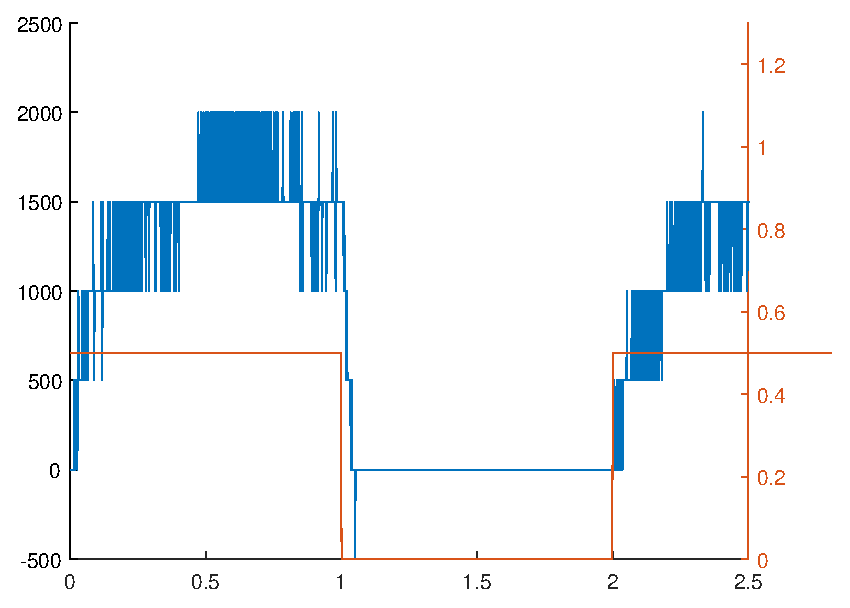
\includegraphics[width=\textwidth]{../Experiments/raw_speed.eps}
        \caption{Raw speed measurements}
        \label{fig:raw1}
    \end{subfigure}
    ~ %add desired spacing between images, e. g. ~, \quad, \qquad, \hfill etc.
      %(or a blank line to force the subfigure onto a new line)
    \begin{subfigure}[b]{0.4\textwidth}
        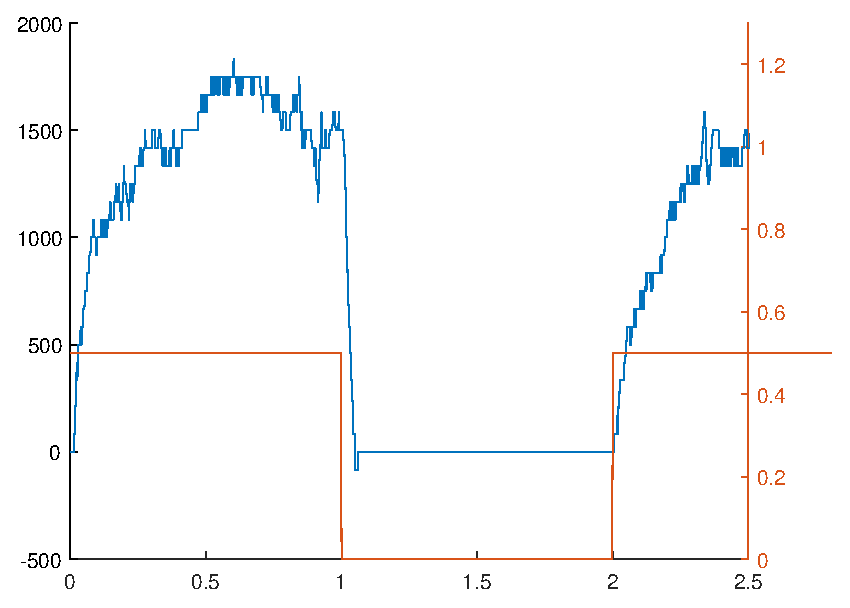
\includegraphics[width=\textwidth]{../Experiments/filtered_speed.eps}
        \caption{Filtered speed measurements}
        \label{fig:filter1}
    \end{subfigure}
%    \caption{Pictures of animals}\label{fig:animals}
\end{figure}

With this data, we first establish our DC gain, for this we find our steady-state value. In this case, we find a value of 1500 ticks per second, and considering the conversion of $2.28 * 10^{-5}$ meters per ticks, this translates to a speed of 0.1083 meters per second. Therefore, our gain is 0.0684.\\
Next we find our time constant. We consider our steady-state error data ($x_{ss} - x$) and proceed to find a exponential curve fitting using Matlab. This generates the following figure and the following coefficients:
\begin{figure}[!htb]
    \centering
    \begin{subfigure}[b]{0.4\textwidth}
        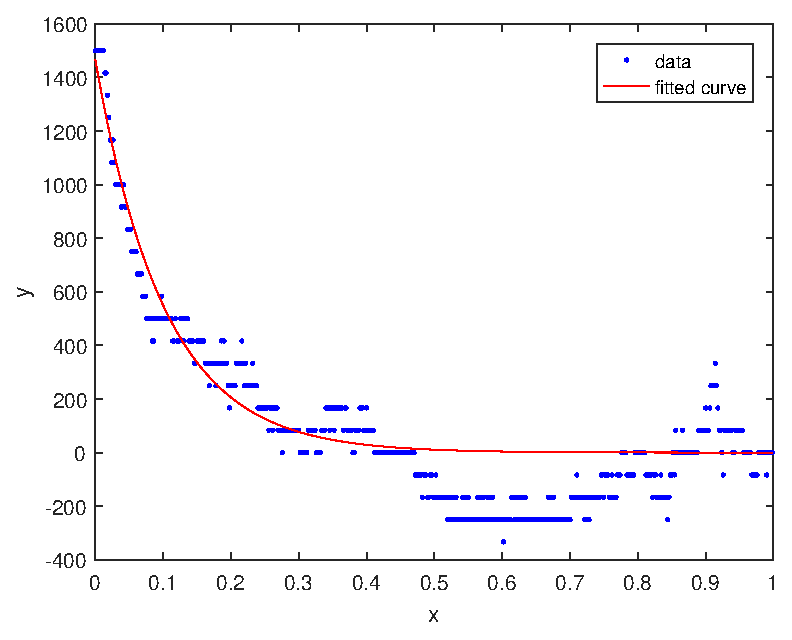
\includegraphics[width=\textwidth]{../Experiments/fitted_data.eps}
        \caption{Exponential curve fitting}
        \label{fig:fit1}
    \end{subfigure}
    ~ \begin{subfigure}[b]{0.4\textwidth}
        \begin{eqnarray*}
            f(x) &=& a*e^{(b*x)}\\
            a &=& 1466\\
            b &=& -9.809\\
            \tau &=& \frac{1}{9.809} = 0.1019
        \end{eqnarray*}
        \caption{Parameter extracted from fit}
    \end{subfigure}
\end{figure}

Finally, we can form our experimental transfer function : $G(s) = \frac{0.0684}{1 + 0.1019s} = \frac{1}{14.62 + 1.49s}$.

\subsection*{3}

As can be seen in figure \ref{fig:com1}, the theoretical and experimental step responses have similar rise times. However, they have wildly different gains; the theoretical gain is approximately 0.225 while the experimental gain is around 0.07.

\begin{figure}[!htb]
    \centering
    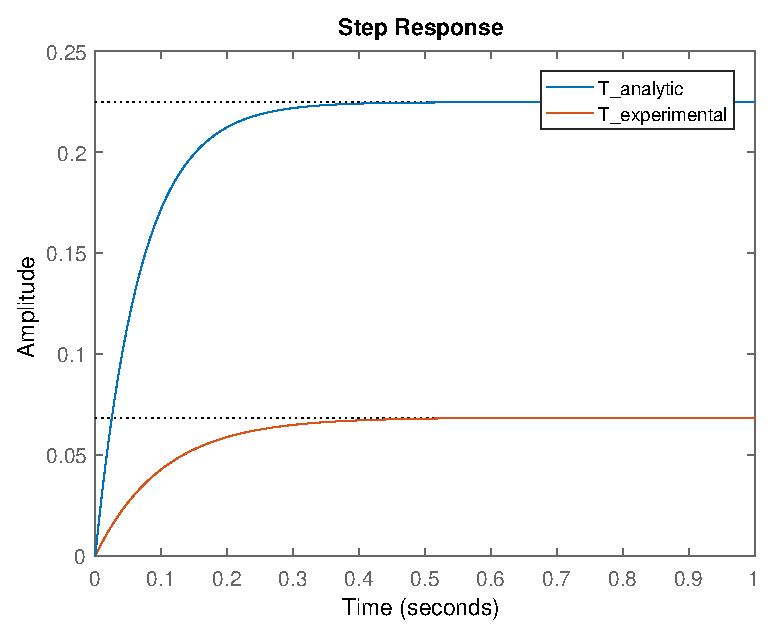
\includegraphics[width=0.8\textwidth]{../Experiments/compare.eps}
    \caption{Comparison of experimental and theoretical model}
    \label{fig:com1}
\end{figure}

Some possible explanations for the differences between the two models are inaccurate simplifications in the theoretical model, experimental noise, aging equipment, and so on. First, our mathematical analysis neglects the effect of friction in the system and the existence of the inductor in the motor. Those will have an impact on the accuracy of the model. Second, our experiment requires we use the derivative of some position encoders. The derivative operation tends to amplify the effect of high frequency signals such as noise. In fact, we can see our raw speed signal is very noisy. As such, graphical approximations and curve fittings will be less precise, leading to increased errors. Finally, the electrical and mechanical components will deteriorate with time. Specifically, the motor's internal resistance, back emf constants, gearbox friction, etc. will change with time and so the design constants in the reference material might not be exact.

\section*{Part 2}
\subsection*{1}
Adding a proportional controller to our system will allow us to control the rise time of the system. To see how, we start from our feedback diagram:

From this diagram, we can derive the following equation:
\begin{equation}
    V = K_p(X_d-X)
\end{equation}
And we know our open loop transfer function $\frac{V}{X}=\frac{1}{As^2+Bs}$. We will replace our voltage equation and isolate $\frac{X}{X_d}$
\begin{eqnarray*}
    \frac{X}{K_p(X_d-X)}&=&\frac{1}{As^2+Bs}\\
    (As^2+Bs)X &=& K_p(X_d-X)\\
    (As^2+Bs + K_p)X &=& K_pX_d\\
    \frac{X}{X_d} &=& \frac{K_p}{As^2+Bs + K_p}
\end{eqnarray*}

We can look at our characteristic equation and normalize it:
\begin{equation}
    s^2 + \frac{B}{A}s + \frac{K_p}{A}
\end{equation}
In this form, it is obvious that $\omega_n^2 = K_p/A$. So we can say that $\omega_n = \sqrt{\frac{K_p}{A}}$. We also see that $\frac{B}{A} = 2\zeta\omega_n$. We isolate $\zeta = \frac{B}{2\omega_nA}$.

We can compute the values for the coefficients using the theoretical parameters and the experimental values calculated in part 1. This yields the following results:



\begin{figure}[!htb]
    \centering
    \begin{subfigure}[b]{0.4\textwidth}
        \begin{tabular}{|l|l|l|l|}
            \hline
            $K_p$ & 20 & 100 & 200 \\\hline
            $\omega_n$ & 8.0687 & 18.0422 & 25.5155\\\hline
            $\zeta$ &  0.8980 & 0.4016 & 0.2840\\\hline
        \end{tabular}
        \caption{Theoretical values of $\omega_n$ and $\zeta$}
        \label{fig:theo2}
    \end{subfigure}
    ~ \begin{subfigure}[b]{0.4\textwidth}
        \begin{tabular}{|l|l|l|l|}
            \hline
            $K_p$ & 20 & 100 & 200 \\\hline
            $\omega_n$ & 3.6637 & 8.1923 & 11.5857\\\hline
            $\zeta$ & 0.6080 & 0.2719 & 0.1923\\\hline
        \end{tabular}
        \caption{Experimental values of $\omega_n$ and $\zeta$}
        \label{fig:exp2}
    \end{subfigure}
\end{figure}

In both cases, we can see that increasing the proportional gain increases the natural frequency of the system and reduces the damping coefficient. This results in a shorter rise time for our system, as well as a lower steady-state error. However, this also means our system overshoot will be greater and will oscillate more before settling.

\subsection*{2}
In order to determine the effect of the proportional gain on the response of the system, we implemented a closed loop system with a proportional gain in Simulink. The testbench we created is illustrated in figure \ref{fig:test2}.

\begin{figure}[!htb]
    \centering
    \includegraphics[width=0.8\textwidth]{part2_schematic.PNG}
    \caption{Closed loop proportional controller}
    \label{fig:test2}
\end{figure}

We ran this test bench with the three coefficients of $K_p$ given. Figure \ref{fig:resp2} shows the measured step responses for the three systems. This figure makes it very easy to see the differences listed above. As previously mentioned, a higher proportional gain will reduce the rise-time and reduce the steady state error, but is also increases the overshoot and oscillations. Interestingly, the difference in the response with $K_p = 100$ and $K_p = 200$ is marginal when compared to the over-damped response with $K_p = 20$. This tells us that our critically damped response cam be achieved with a gain somewhere between 20 and 100.

\begin{figure}[!htb]
    \centering
    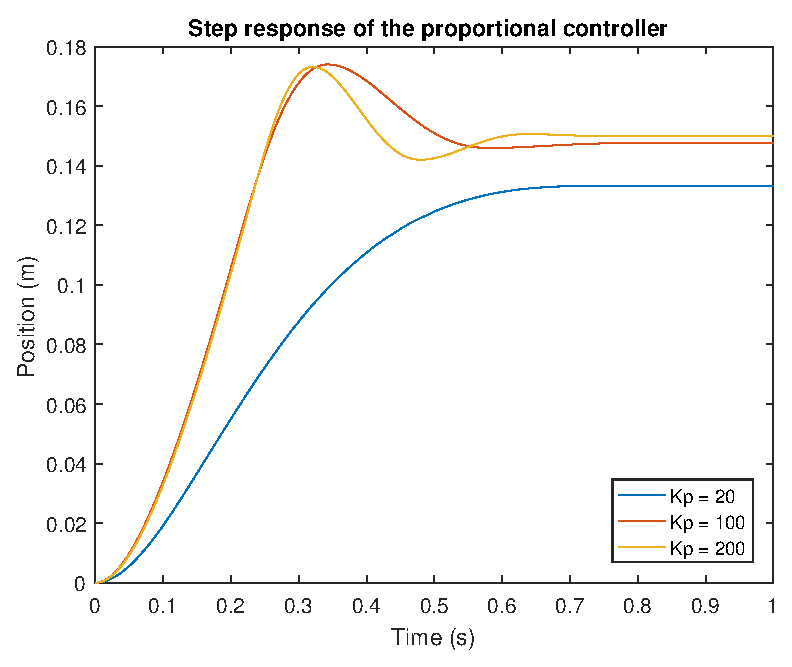
\includegraphics[width=0.8\textwidth]{../Experiments/part2_response.eps}
    \caption{Comparison of step response of proportional controller}
    \label{fig:resp2}
\end{figure}

\section*{Part 3}

\end{document}